

\boxx{\textbf{In this chapter, we learn\dots}
		\itex{
		\item \dots how capital accumulates over time, helping us understand economic growth.
		\item \dots the role of the diminishing marginal product of capital in explaining differences in growth rates across countries.
		\item \dots the principle of transition dynamics: the farther below its steady state a country is, the faster the country will grow.
		\item \dots the limitations of capital accumulation, and how it leaves a significant part of economic growth unexplained.	
}}

\boxx{Required readings:\\ \readsmall \citet[Chapter 11]{Blanchard2013Blanchard}.

Recommended readings:\\ \readsmall \citet[Chapter 10-12]{Blanchard2013Blanchard}
\\ \readsmall \citet[p. 5-29]{Romer2006Advanced}.}

% TODO: \usepackage{graphicx} required
\begin{figure}
	\centering
	\includegraphics[width=0.4\linewidth]{../../../pic/makro/solow}
	\caption{Robert M. Solow: Winner of the Nobel Memorial Prize in Economic Sciences in 1987}\label{fig:rsolow}
	\note{Source: \cite{Storbeck2020Robert}}
	\label{fig:solow}
\end{figure}

\begin{figure}[h]
	\centering
	\begin{center}
		\includegraphics[width=.8\linewidth]{../../../pic/gdp-diff}
	\end{center}
	\caption{GDP per capita over time}\label{fig:growthstick}
	\note{Source: \url{www.core-econ.org}}
\end{figure}





\pbn
%\section{Introduction}



%\zitat{All theory depends on assumptions which are not quite true. That is what make it theory. The art of successful theorizing is to make the inevitable simplifying assumptions in such away that the final result are not very sensitive.\hfill --- Robert M. \citet{Solow1956contribution}}  

%Robert M. Solow born August 23, 1924 and

This chapter focuses on the determinants of economic growth \textbf{in the long run}. In particular, we present a growth model developed independently by \cite{Solow1956contribution} (see \autoref{fig:rsolow}) and \cite{Swan1956Economic} that is called the \textit{Solow-Swan growth model}, the \textit{neoclassical growth model}, or simply the \textit{Solow model}.

\textbf{Long run} means that we are not talking about cyclical movements. Rather, we are talking about long-term trajectories that span decades. Long-term growth models are about real income or real output, and we ignore things that matter a lot in the short run, like inflation or demand. 



\section{Stylized facts}

\exex{Visualization of welfare}{
	\itex{
\item Watch \textit{Hans Rosling's 200 Countries, 200 Years, 4 Minutes - The Joy of Stats - BBC Four}: \tv \url{https://youtu.be/jbkSRLYSojo}
	\item Visit \websmall \url{https://livingcost.org/cost/germany/indonesia} and 
	\item \websmall \url{https://data.worldbank.org/indicator/NY.GDP.PCAP.KD.ZG?end=2022&locations=ID&start=1961&view=chart}. 
}
Please discuss about what led to Indonesia's impressive catch-up growth. Also speculate when this rapid growth might slow down. Moreover, do you think it is possible for Indonesia to attain a GDP per capita similar to that of a Mid-European country like Germany?
}


\pbn
\desx{
	\item[Timing of growth] In \autoref{fig:growthstick}, it's evident that numerous countries have witnessed a form of \textit{hockey-stick} growth.
	Growth take-off occurred at different points in time for different countries:	
	Britain was the first country to experience sustained economic growth. It began around 1650.
	In Japan, it occurred around 1870.
	The kink for China and India happened in the second half of the 20th century. 
	In some economies, substantial improvements in people’s living standards did not occur until they gained independence from colonial rule or interference by European nations.
	
	\item[The Industrial Revolution]
	The Industrial Revolution, also called the Technological Revolution, was a transformative era from the late 18th to 19th centuries. It brought technological advances, like machinery and steam power, that revolutionized manufacturing and led to urbanization. This period reshaped economies, labor, and society, shaping the modern world.

\begin{figure}[h]
	\begin{center}
		\includegraphics[width=.7\linewidth]{../../../pic/lumen}
	\end{center}
	\caption{Lumen-hours per hour of labor}	\note{Source: www.core-econ.org}\label{fig:lumen}
\end{figure}

\begin{figure}[h]
	\begin{center}
		\includegraphics[width=.7\linewidth]{../../../pic/con-world}
	\end{center}
	\caption{A connected World}\label{fig:speednews}
	\note{Source: www.core-econ.org}
\end{figure}

\begin{figure}[h]
	\begin{center}
		\includegraphics[width=.8\linewidth]{../../../pic/cpu-his}
	\end{center}
	\caption{42 Years of microprocessor trend data}\label{fig:cpu}
	\note{Source: \cite{Rusanovsky2019BACKUS}}
\end{figure}
	
	\item[Technology] is the process that uses inputs to produce an output. For example, a technology for making a cake can be described by the recipe that specifies the combination of inputs (ingredients such as flour, labor activities such as stirring, the oven, and the energy) needed to create the output (the cake).
	
	By reducing the amount of work time it takes to produce things, technological changes allowed significant increases in living standards. Figures \ref{fig:lumen}, \ref{fig:speednews}, and \ref{fig:cpu} show the fast development in technology in some areas that play a role in the production process and have an impact on welfare.
		
		\begin{figure}[H]
			\begin{center}
				\includegraphics[width=.6\linewidth]{../../../pic/pop-dev}
				\includegraphics[width=.38\linewidth]{../../../pic/pop-grow}	
			\end{center}
			\caption{World population over time}\label{fig:popstick}
			\note{Source: www.core-econ.org}
		\end{figure}
	
	\begin{figure}[h]
		\begin{center}
			\includegraphics[width=\linewidth]{../../../pic/uk-growth}
		\end{center}\caption{UK GDP growth (1875–2020)}\label{fig:uk-growth} \note{Source: \url{https://www.core-econ.org/the-economy/book/text/13.html}}
	\end{figure}
	
	\item[Economic cycles] \autoref{fig:uk-growth} illustrates the long-term GDP growth of the UK, highlighting its fluctuations and indicating the most severe crisis.
		
	\item[Population growth]	
	\itex{\item Population has also experienced \textit{hockey-stick} growth, see \autoref{fig:popstick}
		\item Growth is slowing down due to the demographic transition\\
		(fall in birth rates > fall in death rates)}
	
	\item[Environmental consequences]	The consequences on the environment stem from heightened production and population growth. This impact manifests globally through climate change and locally through increased pollution in urban areas as well as deforestation. Nevertheless, it's important to recognize that new technologies could potentially hold solutions to these issues. \autoref{fig:temperature} shows some important environmental measures.
}

\begin{figure}
	\begin{center}
		\includegraphics[width=\linewidth]{../../../pic/temp-dev2}
	\end{center}
	\caption{Global atmospheric concentration of carbon dioxide and global temperatures (1750–2019)}\label{fig:temperature}
	\note{Source: \url{https://www.core-econ.org/the-economy/book/text/20.html}}
\end{figure}
%
%\begin{figure}[h]
%	\begin{center}
%		\includegraphics[width=\linewidth]{../../../pic/carbon-dev}
%	\end{center}
%	\caption{Carbon and $CO_2$}\label{fig:carbon}
%	\note{Source: www.core-econ.org}
%\end{figure}

\clearpage





\section{Solow model}

\subsection{Introduction to the Solow model of economic growth}

Watch \tv \url{https://youtu.be/eVAS-t83Tx0}

\boxx{
The nicely animated video is discussing counterintuitive economic growth situations and presents two puzzles: Germany and Japan's rapid growth after World War II despite heavy losses, and China's astonishing growth compared to advanced economies despite having better institutions and more capital. The Solow Model of Economic Growth is introduced to help understand these dynamics and distinguish between "catching up" and "cutting edge" growth. The model simplifies growth factors: labor ($L$), human capital ($L\cdot e$), physical capital ($K$), and ideas ($A$). These inputs work together in a production function to generate output. The production function's abstraction will be further simplified in upcoming videos, starting with an exploration of how capital contributes to economic growth.
}

Here is a transcript of the video:

\zitat{
Here's a fact about economic growth that might seem counterintuitive. During World War II, Germany and Japan suffered heavy losses. Millions of
people were killed. Entire cities were flattened. Roads, bridges, factories, and other resources critical to an economy were destroyed. Yet, following World
War II, Germany and Japan both grew quickly. In fact, they grew much faster than did the United States. Many people wondered what was going on. Why were the losers of the war growing faster than the winners? Here’s another puzzle. In the past several decades, China has been growing at
astonishing rates of growth -- 7 to 10 \% per year. Remember, at those rates, the standard of living -- it's doubling every 7 to 10 years. In contrast, in the
advanced economies, like the United States, Canada, or France, they're growing around 2\% per year, doubling only once every 35 years. So here's the
puzzle. In the previous talks, we said that the way to get a high standard of living and economic growth is to have good institutions, like property rights,
honest government, political stability, a dependable legal system, and competitive and open markets. But in each one of these cases, there's no question
that the advanced economies have better institutions than does China. Plus, the advanced economies -- they've got more human and physical capital. So
if the advanced economies have got better institutions and more capital, why are they growing slower than China? To solve these puzzles, we're going to
be drawing on an important economic model the Solow Model of Economic Growth, named for Robert Solow, who won the Nobel Prize. The Solow Model
will help us to better understand the dynamics of growth. The Solow Model is also going to help us to draw a distinction between two types of growth
catching up growth and cutting edge growth. As we'll see, catching up can be much faster than growing on the cutting edge. Now, you might ask,
``What's an economic model?'' An economic model is a simplified framework that helps us to understand a more complex reality. We're going to be using
a super simple version of the Solow Model that boils economic growth down to just a few key variables and some basic mathematics. Now, although it's
simple, the Solow Model can provide us with some deep insights into the causes of growth. A key part of the model is a production function -- a simplified
description of how resources, inputs, are used to produce output. So let's take a look at some of the inputs into our production function. The first key
input is us, people. We use the letter $L$ to represent labor. The more educated people are, the more effective their labor. So we can multiply $L$ by $e$ for
education. Together, these two variables represent human capital. Next is physical capital, represented by the letter $K$. $K$ is all of our factories, and tools,
and so forth.
Last, but certainly not least, is ideas, represented by the letter $A$. $A$ represents all of our knowledge about how to combine capital and labor to produce
valuable output. Everything from how to transport stuff without carrying it on your back, to how to keep diseases from spreading, to how to add up,
numbers in a fraction of a second. $A$ is ideas, and better ideas mean that we can get more bang for our buck, more output from the same inputs of
 capital and labor. We can think of human capital, physical capital, and ideas being used together to produce output. That's the idea of our production
function. Now, right now our production function is very abstract. But in future videos, we’re going to boil it down even more and make our production
function concrete. We're going to start in the next video by taking a closer look at how capital -- machines, factories, roads, and so forth -- how capital
contributes to economic growth. Let's dig in.
}

\subsection{\tv \textit{The Solow Model and the Steady State}}

Watch \tv	\url{https://youtu.be/LQR7rO-I96A}

	
	Transcript of the video:
	
\zitat{
Let's continue our exploration of the Solow Growth Model. In our last video, we covered how physical capital faces the iron logic of diminishing returns.
Now let's turn to another unfortunate aspect of physical capital: capital rusts. Roads get potholes and need to be repaired, tools wear out, trucks break
down. In short, we say that capital depreciates. Now let's put the amount of capital on the horizontal axis and the amount of depreciation on the vertical
axis. We can then model the relationship like this. Depreciation increases at a constant rate as the capital stock increases. The more capital you have, the
more capital depreciation you have. Now let's add a new aspect to our model. Where does the money for capital accumulation come from? From savings
and investment. When we create economic output, we can either consume it or save it. What we don't consume can be saved and invested in new
capital. So suppose we invest a constant fraction of our output. Let's say we devote of every units of output or 30\% of output to investment. We can now
add an investment curve to our graph. It'll mimic the shape of the output line since investment is just a constant fraction of output. Notice that our first
units of capital -- they’re very productive and so they create a lot of output and thus also a lot of investment. But as we add more and more units of
capital, we get less output and also less investment. That's the iron logic of diminishing returns once again. Now let's put investment and depreciation on
the same graph. Depreciation is growing at the same rate as the capital stock grows. Each new unit of capital creates an equal amount of depreciation.
Now notice that when investment is greater than depreciation, that means the capital stock must be growing. We're adding more units of capital than
are depreciating. But as the capital stock grows -- investment and depreciation -- they're on a crash course to intersect. When this happens, we've
reached what is called the Steady-State Level of Capital. The steady-state is the key to understanding the Solow Model. At the steady-state, an
investment is equal to depreciation. That means that all of investment is being used just to repair and replace the existing capital stock. No new capital is
being created. Now remember, we've assumed that all the other variables in the model -- they're not changing. So if the capital stock isn't growing,
nothing is growing. In other words, when we reach the Steady-State Level of Capital we've also reached the Steady-State Level of Output. Now suppose
you ended up on the other side of the steady-state point -- over here. You'd find that depreciation is greater than investment. That means some of the
capital stock needs repair, but there isn't enough investment to do all of the needed repairs, so the capital stock shrinks, pushing you back towards the
steady state. So to the left of the steady-state we have investment greater than depreciation and the capital stock is growing. To the right of the steady-state we have
the opposite -- depreciation is greater than investment, and the capital stock -- it's shrinking. Either way, we always end up moving towards the steady-state. let's go back to our earlier example of Germany after the end of World War II. Since the capital stock is low, it's also very productive and we get a
lot of output from the first new roads and factories after the war. We've already mentioned that point. But in addition, we now see that when the capital
stock is very productive and producing a lot of output, we will also be producing a lot of investment. So in the next period the capital stock will be even
bigger than before and we'll get even more output. Plus, since the capital stock is low, we don't have much depreciation to take care of. So with the
investment, it will mostly be generating new capital, not replacing old capital. Now over time, however, both of these forces -- they weaken. The returns
to capital diminish and depreciation eats up more and more of investment. A country with a lot of roads, and bridges and factories -- it's doing well, but it
also has to invest a lot just to maintain all those roads and bridges and factories. And this is exactly what we saw in Germany and Japan after World War
II. Growth rates started out very high, but as those countries caught up, growth rates declined. Now perhaps our friend $K$ still has one more trick up his
sleeve to get the economy growing. What if we started to save more of our output? A higher savings rate shifts the investment curve up like this. Now
investment is higher than depreciation, so we're adding to the capital stock and the economy is back to growing. However, you can see that the same
dynamic exists as before. The iron logic of diminishing returns means that we'll again end up at a new steady-state level of capital. The higher savings
rate -- it spurs growth for a time and it does increase the steady-state level of output. But, at the new steady-state, investment once again equals
depreciation and we get zero economic growth. Accumulation of physical capital can only generate temporary growth. In our next video, we'll take a look
at how human capital influences growth.
	}

\subsection{\tv \textit{The Solow Model and Ideas}}

Watch \tv	\url{https://youtu.be/-yPDlowSL1w}

	Transcript of the video:

\zitat{
We've covered a lot of the Super Simple Solow Model. We've looked at the dynamics of capital accumulation, how changes in savings rates influence
growth, and we've looked look at some of the predictions of the Solow Model. One thing we've learned is that the model seems to inevitably predict that we end up in a steady state with no growth. Now, however, we're going to turn to the last of our variables ideas. Can ideas keep us growing? Better ideas
mean that we get more bang for our buck, more output from the same inputs of capital and labor. Alternatively, we can think about this as increasing
our productivity. Henry Ford, for example, took ideas from lots of other industries, like meatpacking, bicycle making, and brewing, and he combined them
in a way that had never before been used in the manufacturing of automobiles. This novel combination of ideas sparked a dramatic increase in
productivity that transformed the world. The same types of processes -- they're continuing today, and in all industries, increasing output per worker
across the economies. So let's go back to our previous graph of capital and output. We can now add ideas as a multiplier. Better ideas multiply the output
from the same capital stock. So, if A increases from 1 to 2, that's a doubling of our productivity. And that shifts the output curve up. When output doubles,
so does investment. Now, once again, investment is greater than depreciation. So we begin accumulating capital once again. And that further boosts our
output. So better ideas spur more output, which creates more investment, which leads to capital accumulation. So better ideas lead to growth in two
ways The increased productivity of a given capital stock, and the increased investment, which increases capital accumulation. Now imagine that ideas
are constantly improving. You'd have continual shifts upward of the output curve. And that means continual shifts upward of the investment curve. We'd always stay to the left of the steady state, and there, we'd continually grow. So growth at the cutting edge -- it's determined by how fast new ideas are
formed, and how much those new ideas increase our productivity. So that's our super simple Solow Model. It combines a model of catching up growth
due to capital accumulation, with a model of cutting edge growth due to idea accumulation.
}



\pbn
\subsubsection{Solow's central question}
Can capital accumulation lead to long-term growth and perpetual improvements in living standards? Formally speaking, can the following circular relationship last forever and lead to sustainable growth in production: $Y\uparrow \rightarrow S\uparrow \rightarrow I\uparrow \rightarrow K \uparrow \rightarrow Y\uparrow \dots$


Robert M. Solow's answer is: No, capital accumulation can boost growth only for some time. The only long-term key to growth is technological progress.

\boxb{\paragraph{\zitat{``Whether you like it or not, history is on our side. We will bury you!''}} This is a quote of Soviet First Secretary Nikita Khrushchev while addressing Western ambassadors at a reception at the Polish embassy in Moscow on November 18, 1956 \citep{Magazine1956Foreign}.
	
	In the 1950s, the Soviet Union launched a growth offensive with extremely high investments, primarily in heavy industry. History was not really on his side as far as we can judge that.
}




\pbn
\section{The formal Solow model}

There are many different versions of the Solow model out there. Each comes with its unique way of of writing things down, which might puzzle newcomers who are trying to understand it.

To make your reading of research easier, let me introduce you to the approach taken by \citet[p. 5-29]{Romer2006Advanced}. In his widely-recognized book for graduate students, he presents the classic form of the model. Despite its challenging aspects, it's designed to be quite comprehensible. 

\subsection{Production}

The heart of any theory of growth is a production function (PF) as it describes how output is made out of different factors of production. Production
in the Solow model takes the form 
\begin{align}
	Y(t)&=f(K(t), A(t)L(t))
\end{align}
where $Y$ is output, $K$ is the input of physical capital (buildings and machines), $L$ is the input of labor, and $A$ is \textit{knownledge} or the \textit{effectiveness of labor}. Time $t$ does not enter production directly, but only through $A$, $K$, and $L$. As $A$ and $L$ enters multiplicatively, $AL$ is usually interpreted jointly as \textit{effective labor}. 

For convenience, the time argument ($t$) will henceforth be dropped and the PF can rewritten:
\begin{align}
Y &= F(K,AL)
\end{align}

\pbn
\subsubsection{Constant returns to scale}

If output changes by the factor $c$ when every production factor is multiplied by $c$, then the production function has constant returns to scale (CRS). Production in the Solow model is assumed to take place at constant returns to scale:
\begin{align}
	f(c\cdot K, c \cdot AL)&=c \cdot f(K, AL) \qquad \text{for all } c\geq 0
\end{align}

\pbn
\subsubsection{Intensive form}
CRS allows us to work with the PF in \textit{intensive form}\footnote{\textbf{Why do we need the intensive form here?}:
The intensive form is just a special way to look at a production function and to analyze its factors of production. Here, we simply re-write the PF into the \textit{intensive form} so that we only need to consider only one factor of production, that is, the capital per unit of effective labor $\frac{K}{AL}$. That will be very useful in the further course of the analysis. Of course, the new variables $y=\frac{Y}{AL}$ and $k=\frac{K}{AL}$ are not of interest in their own right. Rather, they are tools for learning about the variables we are interested in. As we will see, the easiest way to analyze the model is to focus on the behavior of $k$ rather than to consider directly the behavior  of the two arguments of the production function, $K$ and $AL$. 

\pbn
To see the intuition behind the intensive form, think of dividing the economy into $AL$ small economies, each with 1 unit of effective labor and $\frac{K}{AL}$ units of capital. Since the production function has constant returns, each of these small economies produces $\frac{1}{AL}$ as much as is poroduced in the large, undivided economy. Thus, the amount of output per unit of effective labor depends only on the quantity of capital per unit of effective labor, and not on the overall size of the economy. \citep{Romer2006Advanced}} setting $c$ to  be $\frac{1}{AL}$:
\begin{align}
	f\left(\frac{1}{AL}\cdot K, \frac{1}{AL} \cdot AL\right) &=\frac{1}{AL} \cdot f(K, AL) \\
\Leftrightarrow	f\left(\underbrace{\frac{K}{AL}}_k, 1\right) &=  \underbrace{\frac{Y}{AL}}_y\\
 F(k)&=y,
\end{align}
where $k$ is defined as $\frac{K}{AL}$ and denotes the amount of capital per unit of effective labor and $y$ is defined as $\frac{Y}{AL}$ and denotes the output per unit of effective labor.

\pbn
\subsubsection{Inada conditions}
The intensive form PF is assumed to satisfy\footnote{\textbf{Why does the PF needs to satisfy these conditions?}: These assumptions are also known as the \textit{Inada conditions} determine the shape of the production function. These assumptions guarantee the stability of an economic growth path in a neoclassical growth model. While we can loosen the assumption of $f(0)=$ with a loss of generality, it would not make sense to assume $f'(k)<0$ because that would mean the more capital we employ in an economy the less output we generate which would be counter-intuitive and crazy to assume. Also, it would be not intuitive to assume or $f'(k)=0$  as this would mean capital has no impact on production. The second derivation is more interesting: Assuming $f''(k)<0$ means that we do \textbf{not} have economies of scale with respect to capital per effective unit of labor. Thus, all economies will converge to a balanced growth path. If we would assume $f''(k)>0$ that would mean that $f'(k)$ would not fall toward zero as $k$ becomes large and hence the actual investment line, $sf(k)$, would not fall below the break-even investment. That would mean that the growth rate would go to infinity which of course makes no sense. \citep{Romer2006Advanced}}
\begin{align}
	f(0)&=0,\\
	f' (k)&>0,\\
	f'' (k)&<0.
\end{align}
A PF that satisfying these assumptions is shown in figure \autoref{fig:inadapic}. 
A nice series of lecture units explaining the Solow model can be found here: \tv \url{https://youtu.be/b5Yi-ZhFwKw}

\begin{figure}\centering
\begin{tikzpicture}[scale=0.4]
	\draw[thick,<->] (0,9) node[above]{f(k)}--(0,0)--(9,0) node[right]{$k$};
	\node [below left] at (0,0) {$0$};
	%\draw(0,0)--(9,9) node[right]{$\delta k$};
	\draw(0,0) ..controls (1,5) and (5,6) .. (9,7) ;
\end{tikzpicture}
\caption{An intensive-form PF with positive but diminishing marginal returns}\label{fig:inadapic}
\end{figure}

\pbn
\subsubsection{Cobb-Douglas function}
The function 
\begin{align}
	f(K, AL)&=K^\alpha(AL)^{1-\alpha}
\end{align}
is a well-received PF named after \citet{Cobb1928Theory} that 
\enux{
\item can be written in the intensive  form by dividing both inputs by $AL$:
\begin{align}
	f(k)&=f\left(\frac{K}{AL},1\right)=\left(\frac{K}{AL}\right)^\alpha=k^\alpha
\end{align}
\item satisfies the Inada conditions:\footnote{Alternatively, this can be done also without the intensive form: 	If $K=0$ or $L=0$, $F(K,L)=0$. Check for positive but diminishing returns:
	\begin{align*}
		\frac{\partial F}{\partial L}&=\frac{1}{2}K^{\frac{1}{2}}L^{-\frac{1}{2}}>0 
		\quad 	\text{and} \quad	\frac{\partial^2 F}{\partial L^2}=-\frac{1}{4}K^{\frac{1}{2}}L^{-\frac{3}{2}}<0 \rightarrow \checkmark \text{positive and diminishing}
		\\
		\frac{\partial F}{\partial K}&=\frac{1}{2}K^{-\frac{1}{2}}L^{\frac{1}{2}}>0
		\quad 	\text{and} \quad	\frac{\partial^2 F}{\partial K^2}=-\frac{1}{4}K^{-\frac{3}{2}}L^{\frac{1}{2}}<0 \rightarrow \checkmark \text{positive and diminishing}
\end{align*}}
\begin{align}
	f(0)&=0\\
	f' (k)&=\alpha k^{\alpha-1}>0,\\
	f'' (k)&=-(1-\alpha)\alpha k^{\alpha-2}<0,\quad \textnormal{and} 
\end{align}
\item has CRS:
\begin{align}
	f(c K, cAL)&=(cK)^\alpha(cAL)^{1-\alpha}\\
	&=c^\alpha c^{1-\alpha}K^\alpha(AL)^{1-\alpha}\\
	&=c \underbrace{K^\alpha (AL)^{1-\alpha}}_{f(K, AL)}\\
	&=c Y
\end{align}
}

\pbn
\subsection{Evolution of production factors}

\subsubsection{L and A}
Assume the initial levels of $K$ and $L$ are given and that they continuously change over time.
\begin{align}
	\frac{d L(t)}{d t}&=\dot{L}(t)\\
	\frac{d A(t)}{d t}&=\dot{A}(t).
\end{align}
Further assume that labor grows constantly with rate $n$ and knowledge with $g$:
\begin{align}
	\dot{L}(t)&=nL(t) \Leftrightarrow n=\frac{\dot L(t)}{L(t)}\\
\dot{A}(t)&=gA(t) \Leftrightarrow g=\frac{\dot A(t)}{A(t)}.
\end{align}

As the evolution of labor and knowledge are assumed to be exogenous, we should analyze the evolution of $K$.

\pbn
\subsubsection{K}
Changes in the capital stock are explained with
\begin{align}
	\dot{K}(t)&=sY(t)-\delta K(t),\label{eq:Kdot}
\end{align}
where $sY$ is the fraction of output that is devoted to investment and $\delta$ is the capital depreciation rate, both are exogenous and constant. All output that is not invested in the capital stock, $(1-s)Y$, is consumed as we assume a closed economy here. Both $s$ and $\delta$ are exogenous and constant parameters. 

\pbn
\subsubsection{Evolution of $k$}
To see the dynamics of $k$, that is, $\dot{k}$, we need to consider $\frac{d \left(\frac{K}{AL}\right)}{d t}$ which is a bit tedious to derive that as you need the two derivation rules $$\left(\frac{w}{h}\right)'=\frac{w'\cdot h - w \cdot h'}{h^2}$$  and $$(ab)'=a'\cdot b + a \cdot b'$$ to get with dropping the time argument, $t$, 
\begin{align}
\dot{k}=	\frac{d \left(\frac{K}{AL}\right)}{d t} &= \frac{\overbrace{\dot{K}}^{w'} \cdot \overbrace{AL}^{h} - \overbrace{K}^{w} \cdot \overbrace{(\overbrace{A\dot{L}}^{a'\cdot b}+\overbrace{L\dot{A}}^{a\cdot b'})}^{h'}}{\underbrace{(AL)^2}_{h^2}}\\
%	&=\frac{\dot{K} \cdot AL - K \cdot (A\dot{L}+L\dot{A})}{(AL)^2}\\
	&=\frac{\dot{K}}{AL}-\frac{K}{(AL)^2} \left[A\dot{L}+L\dot{A}\right]\\
	&=\frac{\dot{K}}{AL}-\frac{K\dot{L}}{ALL}-\frac{K\dot{A}}{AAL}\\
	&=\frac{\dot{K}}{AL}-\underbrace{\frac{K}{AL}}_k\cdot \underbrace{\frac{\dot{L}}{L}}_n-\underbrace{\frac{K}{AL}}_k\cdot \underbrace{\frac{\dot{A}}{A}}_g	\\
	&=\frac{\dot{K}}{AL}-kn-kg\\
	&=\frac{\dot{K}}{AL}-k(n+g)
\end{align}
Substituting $\dot{K}=sY-\delta K$ from \autoref{eq:Kdot} yields
\begin{align}
	\dot{k}&=\frac{sY-\delta K}{AL}-k(n+g)\\
	&=s\underbrace{\frac{Y}{AL}}_{y\equiv f(k)}-\delta\underbrace{\frac{K}{AL}}_k-k(n+g)\\
	&=sf(k)-\delta k-k(n+g)\\
		\dot{k}&=sf(k)-k(\delta + n+g)
\end{align}
This is the key equation of the Solow model. The change in the capital stock per effective unit of labor, which is the only factor of production that can cause growth in our model, is determined by $sf(k)$: the \textit{actual investment per effective unit of labor}, and $k(\delta + n+g)$: \textit{the break-even investment}. That is, the investment that must be done to keep $k$ at its existing level. In other words it describes why $\frac{K}{AL}$ gets smaller without investments over time:
\desx{
\item[$\delta k \rightarrow$] capital depreciates (gets less over time)
\item[$nk\rightarrow$] quantity of labor is growing
\item[$gk\rightarrow$] effectiveness of labor is growing 
}

\pbn
\subsection{Steady-state, $k^*$}

The steady-state equilibrium is the point where 
\begin{align*}
	\dot{k}=0.
\end{align*}
At this point, growth is zero as capital per effective labor unit $k$ remains the same over time.  Since output per effective unit of labor $y$ depends on $k$ through the production
function, it is also unchanging.

\begin{figure}[h]\centering
	The	y-axis shows the output per effective unit of labor, $y$.\\
	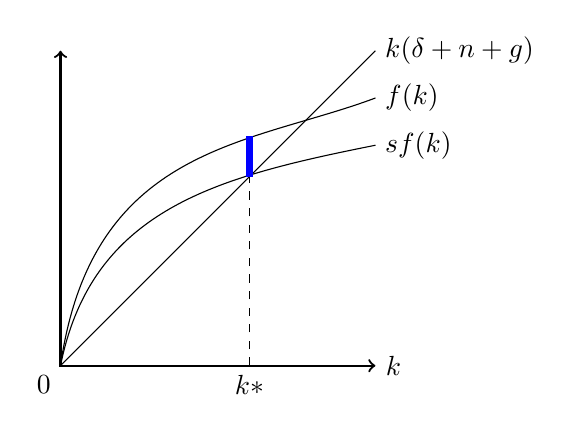
\begin{tikzpicture}[scale=0.4]
		\draw[thick,<->] (0,10) node[above]{}--(0,0)--(10,0) node[right]{$k$};
		\node [below left] at (0,0) {$0$};
		\draw(0,0)--(10,10) node[right]{$k(\delta + n+g)$};
		\draw(0,0) ..controls (1,7) and (6,7) .. (10,8.5) node[right]{$f(k)$};
		\draw(0,0) ..controls (1,5) and (5,6) .. (10,7) node[right]{$s f(k)$};
		%				\draw(0,0) ..controls (1.5,1.5) and (3,3) .. (7,-1) node[right]{$s f(k)$};
		\draw[dashed](6,0)--(6,6) ;
		\draw[solid, line width=1mm	, blue](6,6)--(6,7.3) ;
		\node [below] at (6,0) {$k*$};
	\end{tikzpicture}
	
	
	\begin{tikzpicture}[scale=0.4]
		\draw[thick,<->] (0,10) node[above]{$\dot{k}$}--(0,0)--(10,0) node[right]{$k$};
		\node [below left] at (0,0) {$0$};
		%		\draw(0,0)--(9,9) node[right]{$(\delta-n)k$};
		%		\draw(0,0) ..controls (1,5) and (5,6) .. (10,7) node[right]{$s f(k)$};
		\draw(0,0) ..controls (1.5,1.5) and (3,3) .. (7,-1) node[right]{};
		%		\draw[dashed](6,0)--(6,6) ;
		\node [below] at (6,0) {$k*$};
	\end{tikzpicture}
	\caption{Balanced growth in the Solow model}\label{fig:solowkey}
\end{figure}


\pbn
\subsection{Consumption}
$s f(k)$ is the proportion a country saves and hence invests. 
$k(\delta + n+g)$ refers to how much needs to be invested to keep $k$ stable. 
Thus, the thick blue line denotes the fraction of overall production, $f(k)$, that goes to consumption, $C$, that is
\begin{align}
	C=f(k)-sf(k)
\end{align}
The dashed line is the proportion that is re-invested.
In the steady-state, actual investments equals break-even investment, $(n+g+\delta)k^*$. Thus,
steady-state consumption is given by
\begin{align}
	c^*=f(k^*)-(n+g+\delta)k^*.
\end{align}

\pbn
\subsection{Golden Rule of consumption}
Increased investment in the capital stock can only boost growth until the steady state is reached. Thus, the question arises:  How much should we invest in the capital stock? Well, the only variable we should consider in the long run when deciding on how much to invest from the output, $sf(k)$, is consumption.  The reason is simply that it is consumption not output that defines welfare. Maximal steady-state consumption, $C^{**}$, is given by 
\begin{align}
	\frac{\partial C^*}{\partial s}=\underbrace{\left[ f'(k^*)-(n+g+\delta)\right]}_{\textnormal{Golden Rule}}\frac{\partial k^*}{\partial s}.
\end{align}
The \textit{golden rule} states that consumption is maximized at the point when the slope of the output function, $f(k)$, in the upper panel of \autoref{fig:solowkey} equals $n+g+\delta$.


%\begin{figure}[ht!]
%	\centering
%	\begin{tikzpicture}
%		\begin{axis}[ylabel = {Output per unit of effective labor}, xlabel={$k$}, yticklabels={,,},xticklabels={,,},scale=1.75, xmin=0, ymin=0]
%			\addplot[domain=0:1.000,black]
%			{.75*x} node at (axis cs: .85,.750) {$(n+g+\delta)k$};
%			\addplot[domain=0:1.000,black,samples=1000]
%			{.6299*x^(1/3)} node at (axis cs: 1.050,.650) {$sf(k)$};
%			\addplot[domain=0:1.000,black,samples=1000]
%			{.90*x^(1/3)} node at (axis cs: 1.050,.900) {$f(k)$};
%%			\addplot[domain=0:1000,black,dashed]
%%			coordinates{(500,714) (500,0)};
%%			\addplot[domain=0:1000,black,dashed]
%%			coordinates{(400,663) (400,0)};
%%			\addplot[domain=0:1000,black,dashed]
%%			coordinates{(300,602) (300,0)};
%%			\addplot[domain=0:1000,black,dashed]
%%			coordinates{(600,759) (600,0)};
%		\end{axis}
%	\end{tikzpicture}
%	\caption{Actual and break-even investment}
%\end{figure}

%\begin{figure}[ht!]
%	\centering
%	\begin{tikzpicture}
%	\begin{axis}[ylabel = {$\dot{k}$}, xlabel={$k$}, yticklabels={,,},xticklabels={,,},scale=1.5, xmin=0, ymin=0]
%%		\addplot[domain=0:1.000,black]
%%		{x} node at (axis cs: .850,1.000) {$(n+g+\delta)k$};
%		\addplot[domain=0:1.000,black,samples=1000]
%		{x^(3/6)-(x^(5/4))} node at (axis cs: 1.050,.900) {$sf(k)$};
%	\end{axis}
%\end{tikzpicture}
%
%	\caption{Phase diagram for $k$}
%\end{figure}


%	\subsection*{Why do we set $\frac{Y_t}{A_tL_t}=\frac{Y_{t-1}}{A_{t-1}L_{t-1}}$?}



%\pbn
%
%\itex{
%\item Capital deepening alone cannot sustain ongoing growth in per-capita output

%\item Only technological progress can lead to improvements in output per worker

%}

%\solx{Technological Progress}{
%
%}

%\paragraph{Summary}
%
%\itex{
%	\item The Solow model provides a means of understanding the transition of economies over time. 
%	\item Investment is determined by the domestic savings ratio (and by the inflow of capital from abroad). 
%	\item Investment in capital will increase capital per worker and lead to growth. 
%	%	\item In less developed countries, savings are relatively low because incomes are low.
%	\item As the stock of capital rises, the extra output produced from an additional unit of capital falls; this property is called diminishing returns.
%	\item Less developed economies have lower capital-output ratios and grow faster (catch-up growth). 
%}

\pbn
\begin{table}\centering
	\caption{Steady-state growth rates in the Solow model}\label{tab:steadygrowth}
	\begin{tabular}{lcc}\toprule
		Variable & Symbol & Steady-state growth rate\\\midrule\medskip
		labor & $L$ & $n$\\
		knowledge & $A$& $g$\\
		Total output	& $Y=yAL$			& $n+g$\\
		Capital per effective unit of labor & $k=\frac{K}{AL}$ & 0\\\medskip
		Output per effective unit of labor	& $y=\frac{Y}{AL}=f(k)$& 0\\\medskip
		Output per unit of labor 			& $\frac{Y}{L}=yA$	&g\\\bottomrule
	\end{tabular}
\end{table}

\pbn
\subsection{Long-run growth rates}
In the steady state we have a balanced growth path where all variables grow at a constant rate, see \autoref{tab:steadygrowth}.

Sustained growth requires technological progress as can be seen in the table because output per worker is only driven by $g$.


\section{Summary}

\itex{
	\item The steady-state equilibrium is the point where investment spending is the same as spending on depreciation and the capital-output ratio remains constant; at this point, growth is zero.
	\item The Solow model provides a means of understanding the transition of economies over time. 
	\item Less developed economies have lower capital-output ratios with accumulating capital they can generate catch up growth. 
	\item Investment is determined by the domestic savings ratio and by the inflow of capital from abroad. 
	\item Investment in capital will increase capital per worker and lead to growth. 
	\item As the stock of capital rises, the extra output produced from an additional unit of capital falls; this property is called diminishing returns.
	\item In the long run, growth requires technological progress, i.e., output per worker is only driven by $g$ (ideas).
}



\exex{Technological Progress}{
	In the long run capital per effective unit of labor is constant and hence the only way that the capital per worker and in turn output per worker increases is with technological progress. Show it formally.	
}

\solx{Technological Progress}{
	
	%\subsection{Standard of living and technological progress: $\frac{Y}{L}$ grows at $g$}
	
	$Y$ grows at $n + g$ and $L$ grows at $n$, so the quotient grows at the difference: $g$.
	This means that in the steady state, living standards (output per person) grow at the
	rate of technological progress .
	
	
	In the long run capital per effective unit of labor is constant and hence the only way that the capital per worker and in turn output per worker increases is with technological progress. 
	
	In the steady-state $\dot{k}=0$ and hence, we can say that
	\begin{align}
		\frac{Y_t}{A_tL_t}=\frac{Y_{t-1}}{A_{t-1}L_{t-1}}
	\end{align}
	This simple assumes that in the steady state the output per effective unit of labor is constant. That means, it does not change from period $t-1$ to period $t$. Please note that while the output per effective unit of labor is constant in the steady state, the output per unit of labor is not.
	\begin{align}
		\frac{Y_t}{A_tL_t}&=\frac{Y_{t-1}}{A_{t-1}L_{t-1}}\\
		\Leftrightarrow \frac{\frac{Y_t}{L_t}}{\frac{Y_{t-1}}{L_{t-1}}}&=\frac{A_t}{A_{t-1}}\\
		\Leftrightarrow \underbrace{\frac{\frac{Y_t}{L_t}}{\frac{Y_{t-1}}{L_{t-1}}}-1}_{\text{growth rate of } \frac{Y}{L}}&=\underbrace{\frac{A_t}{A_{t-1}}-1}_g
	\end{align}
	Thus, in the steady state it is only technological progress, i.e., $g$, that determines per capita growth.\footnote{For simplicity, this was shown in discrete times. However, it also holds true in continuous times.} 
}


\pbn
\exex{Solow Simplified}{
Consider a Solow growth model as introduced in the lecture.  Further assume that population (or labor force) does not growth, $n=0$, and that there is no technological change, $g=0$. The parameters of the model are given by $s=0.2$ (savings rate) and $\delta=0.05$ (depreciation rate).

\abcx{
	\item Name the main assumptions of the Solow model.
	\item Which of the following production functions could we use for the Solow model?
	\itex{
		\item $Y=K^{0.5}L^{0.5}$
		\item $Y=K^{0.4}L^{0.7}$
		\item $Y=K^{1/3}L^{2/3}$
	}
	\item Why it is so important to assume that the production function has constant returns to scale and is concave,  that is,  the marginal returns for the inputs are positive $\frac{\partial f(K)}{\partial K}>0$ but diminishing $\frac{\partial^2 f(K)}{\partial K^2}<0$?
	%\footnote{The Inada conditions are a little stronger than needed for the model:
	%\itex{
	%	\item the value of the function $f(K)$ at $K=0$ is 0: $f(K=0)=0$  
	%	\item the production is concave, i.e.,  the marginal returns for the inputs are positive $\frac{\partial f(K)}{\partial K}>0$ but diminishing $\frac{\partial^2 f(K)}{\partial K^2}<0$
	%	\item $\lim_{x_{i}\to 0}\partial f(\mathbf {x} )/\partial x_{i}=+\infty $
	%}}
	\item Rewrite production function $Y=K^{1/3}L^{2/3}$ in output per effective unit of labor terms.
	\item Find the steady-state level of the capital stock. How high is the growth rate of capital per effective unit of labor in the steady-state?
	\item Calculate the steady-state output per labor.
	\item Sketch the steady-state level of the capital stock in a two-way plot with output per labor and capital per labor on the axes. Mark in the plot how much of the output goes into capital service and how much is left for consumption.
	\item Assume that the saving rate increases to $s=0.3$ calculate the new steady-state level of the capital stock and the corresponding steady-state output per labor. What would be the output maximizing savings rate? 
	\item Discuss if a saving rate of 1 would be a desirable goal. Can you think of a optimal saving rate? What is the \textit{Golden Rule} of Capital Accumulation in the Solow Model? 
	\item The golden rule level of the capital stock maximizes consumption per worker in steady-state. 
	Calculate which capital stock would maximizes consumption per worker in steady-state. 
	\item What is the associated savings rate that must be imposed by a benevolent social planer to have maximized consumption per worker? 
	\item Compare your result in the previous part with the consumption maximizing savings rate. Do citizens need to save more or less? Discuss economic policies that could help the social planner implement real-world situation.
	%depreciation options to save taxes.
	% Knowing that $\dot{k}=sf(k)-\delta k$ 
}
}


%\pbn
%\solx{Solow Simplified}{
%	\abcx{
%\item 
%\begin{enumerate}
%	\item \textbf{Positive and diminishing Marginal Returns to Capital:} The model assumes that as the amount of capital per worker increases, the additional output produced by each additional unit of capital diminishes. In other words, there is a diminishing marginal product of capital.
%	
%	\item \textbf{Constant Returns to Scale in Production:} The model assumes that the production function exhibits constant returns to scale. This means that if both labor and capital are increased by a certain proportion, output will increase by the same proportion.
%	
%	\item \textbf{Exogenous Technological Progress:} The Solow model incorporates technological progress as an exogenous factor that increases the productivity of labor and capital over time. This progress is not explained within the model but is treated as an external input.
%	
%	\item \textbf{Savings and Investment:} The model assumes that a constant fraction of output is saved and invested. The level of savings determines the rate of capital accumulation and, consequently, economic growth.
%	
%	\item \textbf{Full Employment:} The model assumes that the economy operates at full employment, meaning that there is no involuntary unemployment. All available labor and capital resources are effectively utilized.
%	
%	\item \textbf{Closed Economy:} The original Solow model considers a closed economy, meaning it does not consider international trade. It assumes that the economy does not engage in trade with other countries.
%	
%	\item \textbf{Homogeneous Labor and Capital:} The model assumes that all units of labor and capital are identical and can be substituted for each other in production.
%	
%	\item \textbf{Stable Population Growth:} The Solow model often assumes a stable population growth rate. This means that the population is growing at a constant rate, allowing for simplified analysis of the effects of capital accumulation on per capita income.
%	
%	\item \textbf{No Government or Public Sector:} The original Solow model typically does not incorporate the effects of government, taxes, or public spending. These factors are often excluded for simplicity.
%\end{enumerate}
%\item 
%\item 
%\item 
%\item 
%\item 
%\item 
%\item 
%\item 
%\item 
%\item 
%\item 
%	}
%}







% without population growth, $n=0$, and no technological change, $g=0$. The production function is The parameters of
%s = 0.2
%the model are given by
%worker;
%a)
%y
%output per worker;
%c
%consumption per worker;
%Rewrite production function
%Divide both sides by
%L
%δ = 0.05
%(savings rate) and
%1
%2
%Y = K 3 L 3
%i
%(depreciation rate). Let
%k
%denote capital per
%investment per worker.

%}


%\includepdf[pages=-]{files/2020-12-09-Notiz.pdf}


%\section{Institutions matters}
%
%Acemoglu2005Institutions
%North1990Institutions